\chapter{Estado del arte}
\label{cap:capitulo2}

\begin{flushright}
\begin{minipage}[]{10cm}
\emph{Todo progreso depende de la irracionalidad del hombre razonable.}\\
\end{minipage}\\

George Bernard Shaw\\
\end{flushright}

\vspace{1cm}

En el presente capítulo se van a describir algunos de los prototipos y posibles aplicaciones más destacables sobre la detección y mantenimiento del pavimento de las carreteras usando inteligencia artificial y técnicas robóticas. En este estado del arte se revisan más de diez soluciones tecnológicas innovadoras desarrolladas recientemente.
  
%En este estado del arte se revisan cuatro soluciones tecnológicas innovadoras desarrolladas recientemente: el sistema robotizado basado en \textit{Raspberry Pi} para la reconstrucción 3D de baches (Infrarob), el Proyecto HERON para el mantenimiento robótico de carreteras, la plataforma EyesNroad para la detección de deterioros viales mediante \ac{IA}, y el proyecto OMICRON para la automatización del sellado de grietas.


\subsubsection{Sistema de reconstrucción 3D de baches}

\setcounter{footnote}{27} 
Este sistema, explicado en \cite{s23135860}, es creado como parte del proyecto Infrarob\footnote{\url{https://infrarobproject.com/}} y desarrollado en el marco del proyecto europeo Horizon 2020, utiliza una \textit{Raspberry Pi 4B} acoplada a un robot autónomo para capturar imágenes usando una cámara y coordenadas \acs{GPS}, usando el módulo  de baches en carreteras. Las imágenes, tomadas desde diferentes ángulos, son procesadas mediante técnicas fotogramétricas para generar modelos 3D de los baches, permitiendo calcular con precisión el volumen que debe ser rellenado. El sistema también integra un \ac{SIG} para mejorar la gestión del mantenimiento de pavimentos. (Figura \ref{fig:infrarob})

\begin{figure} [h!]
	\begin{center}
		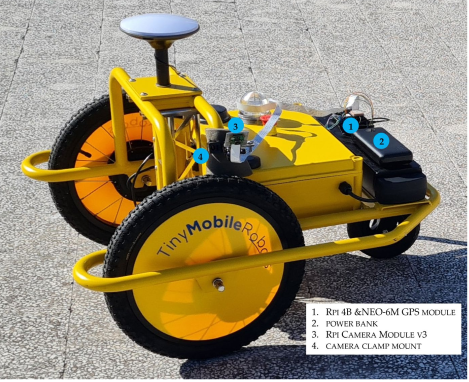
\includegraphics[width=10cm]{figs/infrarob.png}
	\end{center}
	\caption{Robot usado para la reconstrucción 3D de baches}
\label{fig:infrarob}
\end{figure}

Las ventajas de este proyecto son las siguientes: 
\begin{itemize}
	\item \textit{Bajo coste}. Utiliza componentes de bajo coste como: \textit{Raspberry Pi}, \textit{Raspberry Pi Camera} y el módulo \textit{GPS NEO-6M}, que también es \textit{low-cost}. 
	\item \textit{Precisión en la detección}. Capacidad para detectar baches de hasta 75 cm de diámetro y crear modelos 3D precisos.
	\item \textit{Integración con \acs{SIG}}. Facilita la planificación de reparaciones.
	
\end{itemize}\

Las desventajas de este proyecto son las siguientes: 
\begin{itemize}
	\item \textit{Limitaciones climáticas}. No puede operar en condiciones adversas ni durante la noche.
	\item \textit{Uso de software de pago}. Utiliza \textit{ContextCapture}, que es de pago, para el procesamiento fotogramétrico.
	\item \textit{Movimiento circular para detección del volumen}. Una vez detectado el bache, es necesario moverse alrededor de él para que el algoritmo de fotogametría sea capaz de encontrar su volumen, lo que ralentiza el cálculo.
	
\end{itemize}\

\subsubsection{El proyecto Herón}

En \cite{10.1145/3529190.3534746} se habla del Proyecto HERON\footnote{\url{https://www.heron-h2020.eu/}} que también parte del programa Horizon 2020. Este proyecto propone una solución integral para el mantenimiento de infraestructuras viales mediante el uso de vehículos modulares robóticos autónomos y drones. El sistema está diseñado para optimizar la eficiencia y seguridad de las operaciones de mantenimiento, utilizando sensores y escáneres para crear mapas 3D, inteligencia artificial para coordinar flujos de trabajo, y módulos de análisis de imágenes para detectar defectos. Todavía está en etapa de desarrollo. (Figura \ref{fig:heron})


\begin{figure} [h!]
	\begin{center}
		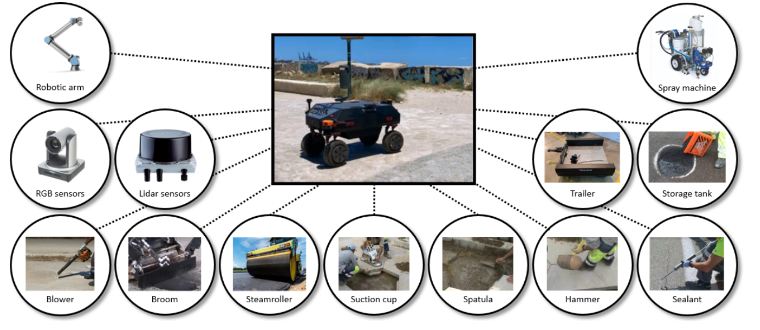
\includegraphics[width=16cm]{figs/heron.png}
	\end{center}
	\caption{Proyecto HERON}
	\label{fig:heron}
\end{figure}

Las ventajas de este proyecto son las siguientes:

\begin{itemize}
	\item \textit{Automatización completa}. Minimiza la intervención humana y reduce riesgos laborales.
	\item \textit{Eficiencia}. El objetivo es mejorar la capacidad y eficiencia de las redes viales.
	\item \textit{Intercambio de datos en tiempo real}. Otro de los objetivos es mejorar la toma de decisiones
	\item \textit{Diseño modular}. Para poder maximizar sus capacidades, facilitar el transporte y reducir los costes de mantenimiento y accidentes.
\end{itemize}\

Las desventajas de este proyecto son las siguientes:
\begin{itemize}
	\item \textit{Coste inicial elevado}. La implementación de tecnologías avanzadas es costosa.
	\item \textit{Dependencia tecnológica}. Requiere una infraestructura tecnológica robusta para su funcionamiento.
\end{itemize}\


\subsubsection{EyesNroad}

EyesNroad es una plataforma que emplea \ac{IA} y \textit{Machine Learning} para identificar baches, señalización y otros deterioros en carreteras a partir de videos capturados por cámaras georreferenciadas instaladas en vehículos. La plataforma genera inventarios detallados y reportes del estado de las carreteras, facilitando el control y mantenimiento de las mismas. Esta aplicación ha sido desarrollada para participar en los XX premios de conservación de carreteras de \ac{ACEX} (año 2024)\footnote{\url{https://www.acex.eu/candidatura-3-4/}}, que ha resultado ganadora en la en la categoría general. Se puede ver su aspecto en la Figura \ref{fig:enr}.

\begin{figure} [h!]
	\begin{center}
		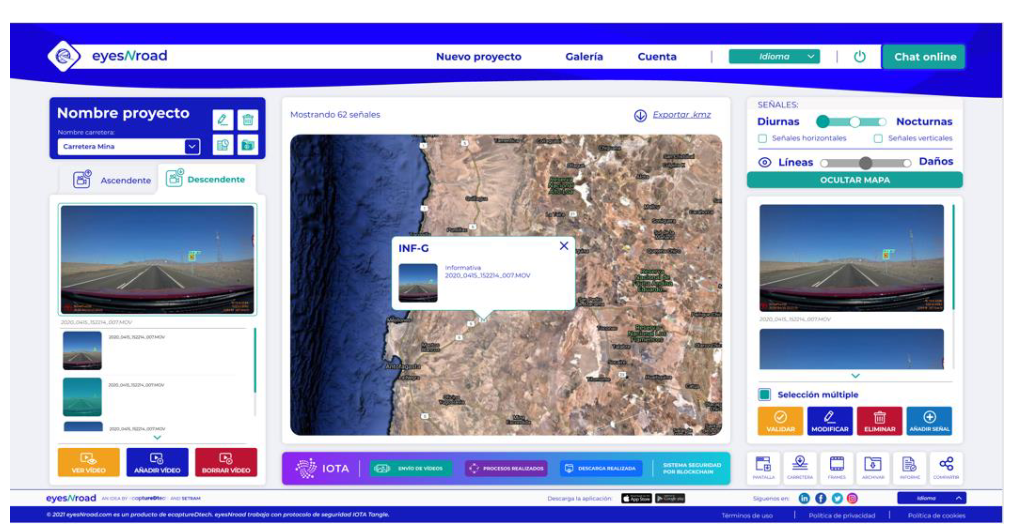
\includegraphics[width=16cm]{figs/enr.png}
	\end{center}
	\caption{Visualización de la señal en un mapa en eyesNroad}
	\label{fig:enr}
\end{figure}


Las ventajas de este proyecto son las siguientes:

\begin{itemize}
	\item \textit{Facilidad de implementación}. Puede utilizarse con cámaras comunes y es compatible con dispositivos móviles.
	\item \textit{Amplia detección}. No solo identifica baches, sino también señalización y otros elementos viales.
	\item \textit{Actualización continua}. La base de datos se amplía constantemente para cubrir más regiones.
	
\end{itemize}\

Las desventajas de este proyecto son las siguientes:
\begin{itemize}
	\item \textit{Limitación geográfica}. Actualmente, su funcionamiento completo está limitado a Portugal.
	\item \textit{Es de pago}. Para cualquier persona que desee usar esta herramienta tiene que asumir los costes.
	\item \textit{No calcula volumen}. La plataforma no ofrece estimaciones del volumen de los baches, lo que podría ser útil para reparaciones.
	
\end{itemize}\


\subsubsection{El proyecto OMICRÓN}

En este proyecto se ha creado un sistema robótico que busca automatizar y robotizar el proceso de sellado de grietas en pavimentos, con el objetivo de eliminar la exposición de los operarios a condiciones peligrosas. El sistema integra un brazo robótico y herramientas de inteligencia artificial para detectar grietas y realizar el sellado de manera autónoma, mejorando así la seguridad y eficiencia en las operaciones de mantenimiento. Esta aplicación ha sido desarrollada para participar en los XX premios de conservación de carreteras de \ac{ACEX} (año 2024)\footnote{\url{https://www.acex.eu/candidatura-12-5/}}, que ha resultado ganadora en la en la categoría asociados. Puedes ver su aspecto en la Figura \ref{fig:omicron}.

\begin{figure} [h!]
	\begin{center}
		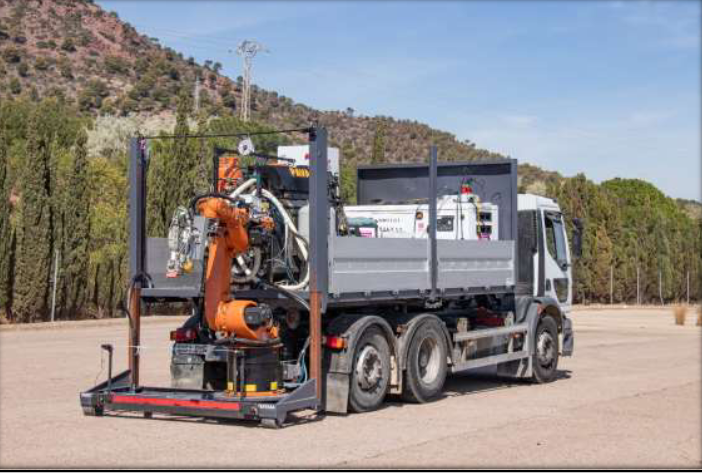
\includegraphics[width=16cm]{figs/omicron.png}
	\end{center}
	\caption{Plataforma robótica diseñada para el sellado de grietas}
	\label{fig:omicron}
\end{figure}

Las ventajas de este proyecto son las siguientes:

\begin{itemize}
	\item \textit{Seguridad laboral}. Elimina la necesidad de que los operarios sufran accidentes de tráfico y tengan contacto con materiales peligrosos.
	\item \textit{Reducción de tiempo}. Debido a la automatización del proceso, se puede reducir el tiempo de intervención.
	\item \textit{Innovación en materiales}. Al invertir en crear un mástico nuevo, se puede operar a temperaturas más bajas.
\end{itemize}\


Las desventajas de este proyecto son las siguientes:

\begin{itemize}
	\item \textit{Es un prototipo}. Todavía está en fase temprana de implementación lo que le impide a los clientes tener una disponbilidad inmediata.
	\item \textit{Alto coste}. Necesita componentes caros para poder llevar a cabo sus objetivos, como un camión o un brazo robótico, entre otros.
	\item \textit{Complejidad técnica}. Ya que se trata de una automatización completa, necesita un alto nivel de precisión y coordinación, lo que supone un gran desafío para su implementación.
\end{itemize}\

\subsubsection{Sistemas de reconstrucción 3D usando SFM y aprendizaje profundo}


Este sistema, descrito en \cite{WANG2023132499}, propone una solución innovadora para la reconstrucción y segmentación 3D de baches en pavimentos. El enfoque aborda las limitaciones de los métodos tradicionales basados en imágenes 2D al utilizar técnicas de fotogrametría para generar perfiles 3D detallados de los baches. El sistema se compone de un método de reconstrucción conocido como Estructura Desde el Movimiento de Pavimentos (PP-SFM) y una red de segmentación 3D, Trans-3D-Seg, que incorpora módulos de transformadores para mejorar la precisión de la segmentación de nubes de puntos 3D. El sistema muestra una alta precisión, con una puntuación F1 del 92.58\% y una precisión general del 93.44\%. Además, se ha demostrado su robustez en diferentes condiciones, como distintas alturas de adquisición y en luz oscura. Otro sistema muy parecido que cumple con todo lo anterior expuesto y que además incorpora un láser para conseguir una segmentación más robusta, está definido en \cite{9345528}.

Las ventajas de estos proyectos son las siguientes:

\begin{itemize}
	\item \textit{Alta precisión}. Los sistemas proporcionan una segmentación precisa de baches, evidenciada por las altas puntuaciones en la precisión y la puntuación F1.
	\item \textit{Robustez}. Los métodos son robustos en diversas condiciones, incluyendo iluminación variable y diferentes alturas de adquisición, lo cual es crucial para aplicaciones prácticas en el terreno.
	\item \textit{Facilidad para la integración}. Ya que los sistemas están preparados para operar en cualquier cámara, facilitan la integración.
	
\end{itemize}\


Las desventajas de estos proyectos son las siguientes:
\begin{itemize}
	\item \textit{Alto coste computacional}. Debido a la complejidad de las aplicaciones, necesitan un procesamiento intensivo. 
	\item \textit{Hardware potente}. La implementación del sistema necesita \textit{hardware} potente y recursos computacionales considerables para el procesamiento de imágenes y la ejecución de modelos de aprendizaje profundo.
	\item \textit{Movimiento circular para detección del volumen}. Una vez detectado el bache, es necesario moverse alrededor de él para que el algoritmo de fotogametría sea capaz de encontrar su volumen, lo que ralentiza el cálculo.
	
\end{itemize}\


En relación a la detección de los baches se pueden encontrar métodos que se pueden enmarcar en tres distintas categorías, descritas en \cite{app12115320}, y que se dividen en: baches detectados por visión, baches detectados por vibración y baches detectados por reconstrucción 3D. Cada categoría tiene una serie de ventajas y desventajas, que es importante conocer a la hora de elegir el tipo de método a usar, y que aparecen descritas en el Cuadro \ref{cuadro:vyd}. A continuación se enumeran alguno de los métodos de cada categoría.

\begin{table}[H]
	\begin{center}
		\begin{tabular}{|c|c|c|}
			\hline
			Métodos & Ventajas & Desventajas\\
			\hline
			%\multirow{3}{4cm}{Métodos} & \multirow{2}{*}[3 mm] {Ventajas} & Desventajas\\
			%\cline{3-3} % línea solo en la tercera columna
			\multirow{2}{*}{Visión} & \multirow{2}{*}{\shortstack{ Más rentable que reconstrucción 3D \\ Adecuada para ciertos baches}} &\multirow{2}{*}{\shortstack{Limitaciones en profundidad \\ Efecta condiciones metereológicas}}\\
			&  &  \\
			\hline
			\multirow{3}{*}{Vibración} & \multirow{3}{*}{\shortstack{ Más rentable de todos \\ Requiere poco almacenamiento\\ Soporta tiempo real}} &\multirow{3}{*}{\shortstack{Limitaciones en formas \\ Depende de la arquitectura }}\\
			&  &  \\
			&  &  \\
			\hline
			\multirow{2}{*}{\shortstack{ Reconstrucción \\ 3D}} &  \multirow{2}{*}{Forma del bache más precisa}  & \multirow{2}{*}{Más caro de todos} \\
		 	&  &  \\
			\hline
		\end{tabular}
		\caption{Ventajas y desventajas de los métodos de detección de baches}
		\label{cuadro:vyd}
	\end{center}
\end{table}


En visión se puede encontrar el método de \cite{app112311229}, que usa modelos de YOLOv4, YOLOv4-tiny y YOLOv5, un dataset total de 665 imágenes (70\% entrenamiento, 10\% validación, 20\% pruebas) y aplicado sobre 
Tesla K80 GPU (12 GB) en \textit{Google Colab}. Otro método es el de \cite{doi:10.1080/14680629.2019.1615533}, que utiliza un modelo de \textit{prepooling CNN} con un dataset de 96,000 imágenes (72,000 entrenamiento, 24,000 pruebas), una precisión optimizada hasta de 0.9825. Todo ello probado sobre un Intel Core i7, 32 GB RAM, GeForce GTX 1080 (8 GB).

En vibración se puede encontrar el método de \cite{s20020451}, que usa un filtro \textit{Butterworth}, un modelo gaussiano mejorado y un algoritmo de \textit{k-nearest neighbor}. Se usan unas 118 muestras de bultos, 174 muestras de planos y 103 de bache. Tiene una precisión de 0.96 para baches y 0.94 para bultos. Se usa un Cavalier con un smartphone Redmi Note 8 Pro con frecuencia de muestreo de 400 Hz. Otro método es el de \cite{7922534} que usa un filtro paso bajo, con transformada de Fourier. Para clasificar se usa un árbol de decisión C4.5 (0.9860), SVM (0.9525)y Naïve Bayes (0.9690). Todo ello se ha probado sobre un smartphone Galaxy Alpha con frecuencia de muestreo de 50 Hz.

Finalmente, para la reconstrucción 3D se puede encontrar el método de \cite{8788687}, que usa visión estéreo de un solo marco, fusión de múltiples marcos, aprendizaje por transferencia con Mask R-CNN y aprendizaje por transferencia con YOLOv2, todo ello usando una GeForce GTX 1080 y un Tesla K80. Otro método es el de \cite{8638822}, que usa un filtro de paso-alto, una ecualización de histograma, una combinación de \textit{waypoints} con triangulación estéreo. Este método ha sido probado en dos webcams A4Tech PKS-732 montadas en un trípode o en la parte trasera de un coche usando un ordenador con sistema operativo Windows.


Los prototipos, métodos y desarrollos tecnológicos presentados demuestran el potencial de la robótica y la \acs{IA} en el mantenimiento y detección de deterioros en el pavimento. Desde la creación de modelos 3D de baches hasta la automatización del sellado de grietas, estos avances no solo mejoran la seguridad y eficiencia de las operaciones, sino que también optimizan la gestión y planificación del mantenimiento vial. No obstante, cada solución presenta desafíos específicos, como la dependencia de condiciones climáticas, la limitación geográfica y los costes asociados, que deben ser considerados al evaluar su implementación en diferentes contextos.\\\\\\ %(hay 3 saltos de línea)

En el siguiente capítulo se va a proceder a definir una serie de requisitos, metodología y un plan de trabajo que se ha seguido para dar solución a los objetivos que se plantean en este proyecto.